\section{Ocean Bottom Seismic (OBS)}

\begin{frame}{Seismic Methods \& Oil Exploration}

    Seismic or acoustic methods measure the travel times of the reflected or refracted waves detected by a series of geophones and are able to estimate the location and depth of the targets.

    \vspace{10pt}

    \begin{columns}[c, onlytextwidth]

        \begin{column}{0.45\textwidth}

            \begin{figure}
                \centering
                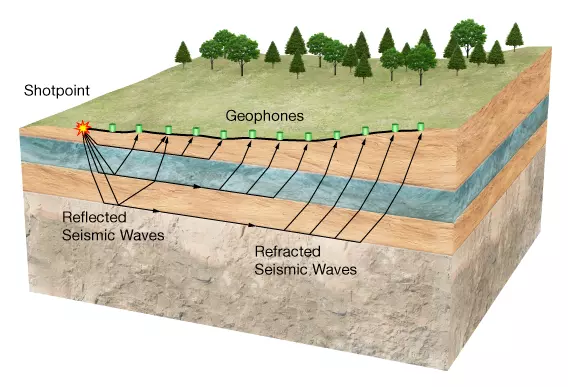
\includegraphics[width=\textwidth]{img/OBS-seimic.png}
                \caption{Seismic method applied from Earth's surface.}
            \end{figure}

        \end{column}

        \hfill

        \begin{column}{0.5\textwidth}

            A \textbf{precise timestamp is required} to measure the travel time of the waves.

            \vspace{10pt}

            Seismic methods are used for oil exploration since they can estimate the location and depth of the oil reservoirs.

        \end{column}

    \end{columns}

\end{frame}



\begin{frame}{Role of CSAC}

    Small short \& medium drifts $\rightarrow$ no GNSS required for nodes synchronization.

    Low battery consumption $\rightarrow$ long-lasting measurements campaigns (weeks or months).

    \begin{figure}
        \centering
        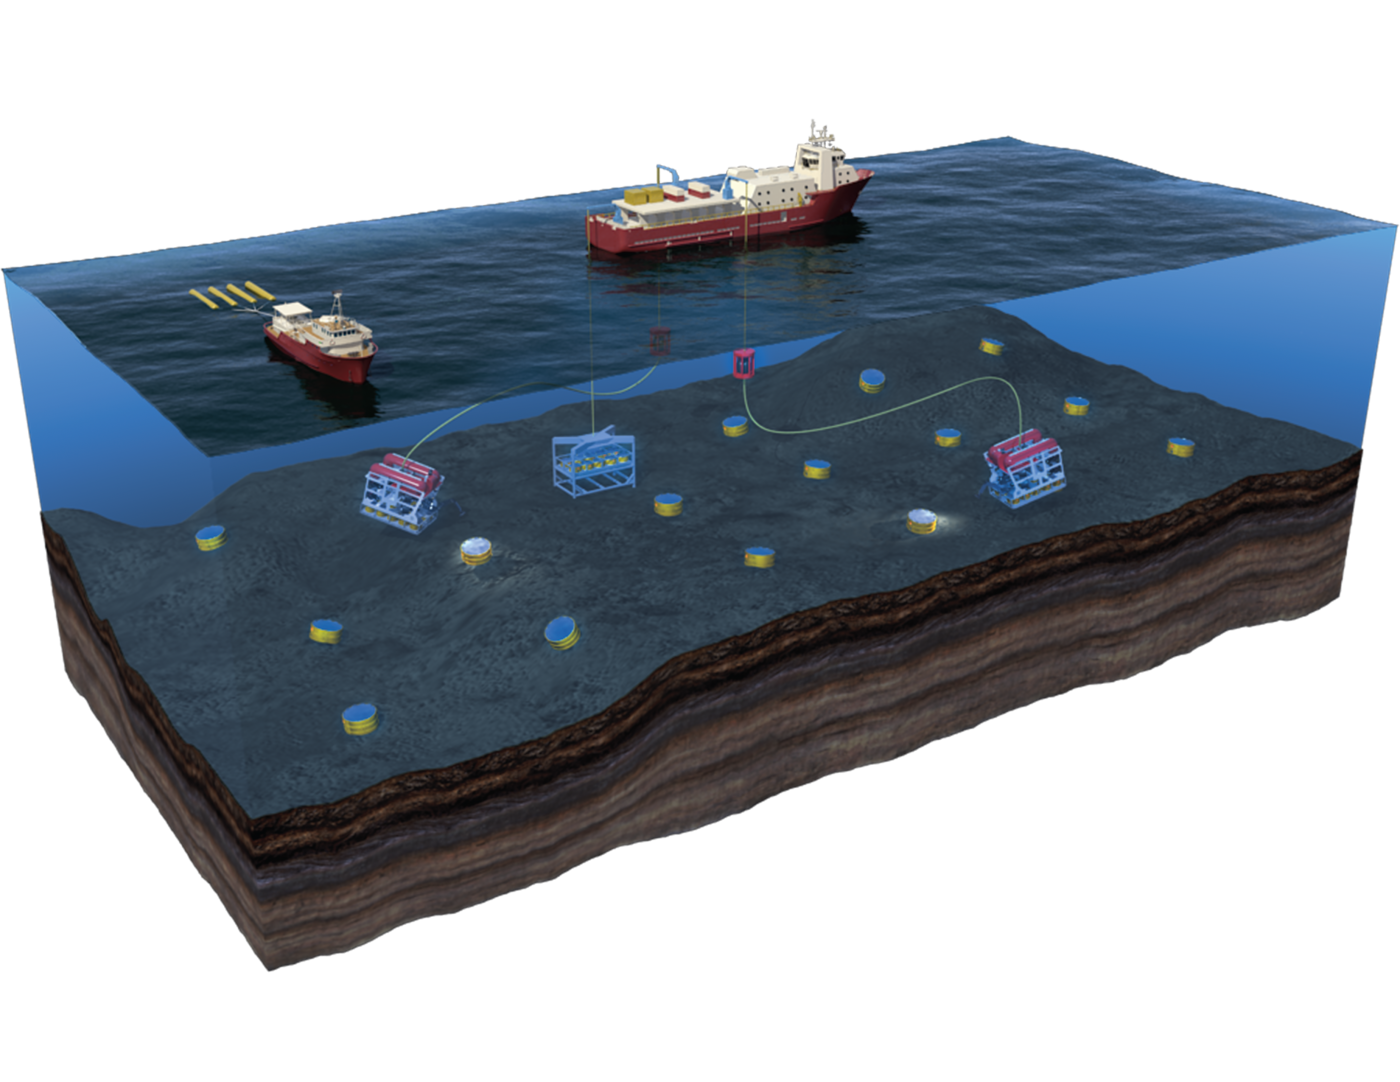
\includegraphics[width=0.5\textwidth]{img/OBS.png}
        \caption{Thanks to CSAC, mapping is now done by placing the geophones on the ocean floor and not on the surface, obtaining more accurate results.}
    \end{figure}

\end{frame}